\documentclass[10pt,a4paper]{article}
\usepackage[margin=2cm]{geometry}
\usepackage{booktabs}
\usepackage{graphicx}
\usepackage{microtype}
\usepackage{hyperref}
\usepackage{tikz}
\usetikzlibrary{arrows.meta,positioning}
% Generated from reproducible experiment outputs. Update after rerunning models.
\newcommand{\LastWAPE}{0.545040}
\newcommand{\DailyWAPE}{0.418006}
\newcommand{\WeeklyWAPE}{0.454876}
\newcommand{\SeasonalWAPE}{0.341780}
\newcommand{\TargetOnlyWAPE}{0.383264}
\newcommand{\FullWAPE}{0.241293}
\newcommand{\SelectedEpoch}{12}
\newcommand{\JenaTempMAE}{2.706}
\newcommand{\JenaTempRMSE}{3.442}
\newcommand{\JenaHumidityMAE}{8.903}
\newcommand{\JenaHumidityRMSE}{11.745}
\newcommand{\JenaNormalizedMAE}{0.431}


\title{Residual LSTM Forecasting for Multivariate Operational Time Series}
\author{Tudor Orza \and Marie Reinhold \and Felix Besser}
\date{Deep Learning, Summer Semester 2026}

\begin{document}
\maketitle

\begin{abstract}
We study hourly multivariate forecasting for 96 anonymized operational units.
The required system predicts 336 hours recursively in blocks of 24 and is
evaluated with weighted absolute percentage error (WAPE). We implement a compact
PyTorch LSTM that predicts corrections to a strong four-week seasonal mean and
uses known future covariates plus learned unit embeddings. On a chronological
336-hour internal holdout, the full model reaches WAPE \FullWAPE, compared with
\SeasonalWAPE\ for the seasonal mean and \LastWAPE\ for last-value persistence.
We additionally evaluate the same model family on hourly Jena climate data for
joint temperature and humidity forecasting. The complete system includes
leakage-safe preprocessing, recursive inference, and a CPU-compatible model
archive.
\end{abstract}

\section{Introduction}
Operational load forecasting supports staffing, capacity planning, and the
early recognition of system pressure. The benchmark contains 96 related but
distinct hourly series, 22 explanatory variables, and one nonnegative target.
At prediction time, covariates for the future interval are known, whereas future
targets are not. The principal challenge is therefore to combine strong daily
and weekly regularities with unit-specific dynamics and externally supplied
signals, while avoiding error accumulation over fourteen recursive blocks.

Our approach deliberately favors a small recurrent model over a much larger
architecture. This choice makes controlled ablations and reproducible CPU
inference practical. The main contributions are (i) a residual LSTM anchored to
a seasonal forecast, (ii) causal missing-value treatment and train-only
normalization, (iii) exact recursive inference for the required 336 hours, and
(iv) a transfer experiment on two-target weather forecasting.

\section{Related Work}
Long short-term memory networks use gated recurrent state updates to preserve
useful information over long sequences \cite{hochreiter1997lstm}. Recurrent
architectures remain a standard tool for nonlinear sequential modeling
\cite{mienye2024rnn}, including robust time-series prediction
\cite{connor1994robust}. Attention-based recurrent models can further separate
feature selection from temporal attention \cite{qin2017dual}; however, our data
volume and reproducibility requirements favor a smaller model.

Seasonal persistence is particularly competitive in short-horizon forecasting.
Instead of asking the neural network to relearn the entire weekly level, we use
a seasonal mean as an explicit inductive bias and train only its residual. This
hybrid strategy makes the neural component focus on deviations explained by
current load, risk, capacity, and calendar variables.

\section{Method}
\subsection{Preprocessing and windows}
For each series, rows are ordered by timestamp and checked for duplicates and
hourly spacing. We reserve the final 336 public training hours for model
selection. Every continuous covariate is standardized with mean and variance
estimated on the remaining training interval only. Cyclic and binary variables
are not standardized. Missing values receive an indicator channel, are
forward-filled within their series, and use the training median only when no
earlier observation exists.

Training examples contain 168 history hours and a 24-hour target block, with a
stride of six hours. Historical targets are standardized per series for the
encoder, but predictions and the L1 objective remain on the original target
scale. Windows begin only after four complete weeks, ensuring that the preferred
seasonal reference is defined.

\subsection{Architecture}
The encoder is a one-layer LSTM with 64 hidden units. Its final hidden state is
processed by Layer Normalization. We concatenate this state with an
eight-dimensional learned series embedding and the covariates known for each
future hour. A shared two-layer decoder predicts a residual for every hour. No
Batch Normalization is used because train-only input scaling and Layer
Normalization are stable for recurrent sequence batches.

\begin{figure}[t]
\centering
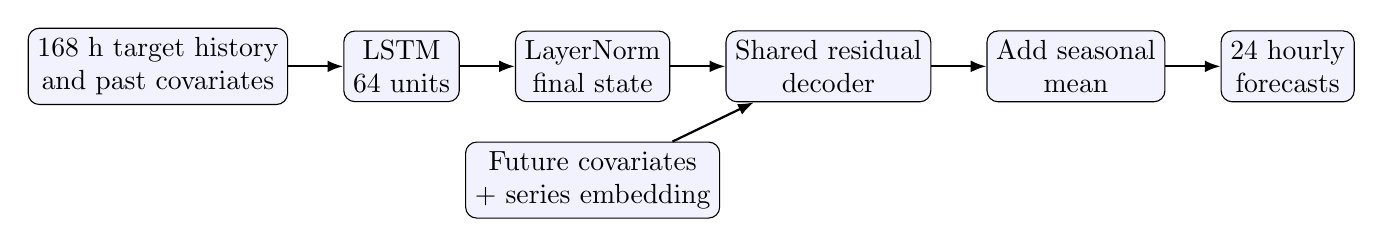
\begin{tikzpicture}[
  node distance=5mm and 7mm,
  box/.style={draw,rounded corners,align=center,minimum height=8mm,fill=blue!5},
  arrow/.style={-{Latex[length=2mm]},thick}
]
\node[box] (hist) {168 h target history\\and past covariates};
\node[box,right=of hist] (lstm) {LSTM\\64 units};
\node[box,right=of lstm] (norm) {LayerNorm\\final state};
\node[box,below=of norm] (future) {Future covariates\\+ series embedding};
\node[box,right=of norm] (decoder) {Shared residual\\decoder};
\node[box,right=of decoder] (add) {Add seasonal\\mean};
\node[box,right=of add] (out) {24 hourly\\forecasts};
\draw[arrow] (hist) -- (lstm);
\draw[arrow] (lstm) -- (norm);
\draw[arrow] (norm) -- (decoder);
\draw[arrow] (future) -- (decoder);
\draw[arrow] (decoder) -- (add);
\draw[arrow] (add) -- (out);
\end{tikzpicture}
\caption{Residual LSTM architecture used for the benchmark. For Jena, the same
encoder and decoder predict two target channels and future inputs contain only
calendar variables.}
\label{fig:architecture}
\end{figure}

The reference forecast averages the values at the corresponding hour in the
four most recent weeks. With less history, it falls back to weekly persistence
and then to the last observation. The decoder output is multiplied by the
per-series target standard deviation and added to this reference. Forecasts are
clamped to zero only at inference. We train with AdamW (learning rate $10^{-3}$,
weight decay $10^{-4}$), batch size 256, gradient clipping at 1.0, and early
stopping with patience five. The maximum is 30 epochs and the fixed seed is 42.

\section{Benchmark Experiments}
\subsection{Evaluation protocol}
The internal holdout exactly matches the required 336-hour forecast length.
Models forecast in 24-hour blocks; predictions are appended to target history
before the next block, so no held-out target is exposed. WAPE is
$\sum_t |y_t-\hat y_t| / \sum_t |y_t|$, aggregated across all units and hours.
After selection, the full model is retrained from initialization on all public
targets for \SelectedEpoch\ epochs.

\begin{table}[t]
\centering
\caption{Internal chronological benchmark results. Lower WAPE is better.}
\begin{tabular}{lr}
\toprule
Method & WAPE \\
\midrule
Last value & \LastWAPE \\
Daily persistence (24 h) & \DailyWAPE \\
Weekly persistence (168 h) & \WeeklyWAPE \\
Four-week seasonal mean & \SeasonalWAPE \\
Target-history-only LSTM & \TargetOnlyWAPE \\
Full multivariate LSTM & \textbf{\FullWAPE} \\
\bottomrule
\end{tabular}
\label{tab:benchmark}
\end{table}

\subsection{Results and ablation}
The target-only LSTM improves over last-value, daily, and weekly persistence,
but it does not beat the four-week seasonal mean. In contrast, the full model
reduces WAPE by approximately 29\% relative to the seasonal baseline and by 56\%
relative to last-value persistence. Since the two neural models share the same
encoder, decoder, optimization, and seasonal reference, this gap is direct
evidence that the supplied covariates provide useful information beyond target
history alone. The full model selected epoch \SelectedEpoch; later epochs
reduced training L1 while validation performance stopped improving, supporting
the early-stopping decision.

\section{Additional Dataset: Jena Weather}
The Jena climate record from the Max Planck Institute for Biogeochemistry
contains ten-minute meteorological observations from 2009--2016
\cite{jena}. We aggregate numerical measurements to hourly means and represent
wind direction with Cartesian wind components. Negative sentinel wind speeds
are marked missing before aggregation. Our targets are air temperature in
degrees Celsius and relative humidity in percent.

The split is chronological: 2009--2014 for training, 2015 for validation, and
2016 for testing. Each origin uses 168 observed history hours to predict 24
hours. Historical meteorological measurements enter the encoder; only hour- and
year-cycle sine/cosine variables are supplied for future timestamps. This
prevents accidental access to future measured weather. The decoder has two
outputs and the loss averages raw L1 error after target-specific normalization
of its residual parameterization.

\begin{table}[t]
\centering
\caption{Jena 2016 test results for the selected LSTM.}
\begin{tabular}{lrr}
\toprule
Target & MAE & RMSE \\
\midrule
Temperature ($^\circ$C) & \JenaTempMAE & \JenaTempRMSE \\
Relative humidity (\%) & \JenaHumidityMAE & \JenaHumidityRMSE \\
\bottomrule
\end{tabular}
\label{tab:jena}
\end{table}

The mean normalized MAE is \JenaNormalizedMAE. Daily, weekly, and last-value
baselines are evaluated at the same origins. This experiment tests whether the
architecture's central idea---recurrent history encoding plus a seasonal
reference---transfers when the number, scale, and meaning of targets change.

\section{Relation to the Expos\'e and Limitations}
The final method follows the expos\'e's choice of an LSTM and its proposed daily
and weekly baselines. Several details changed after inspecting the released
data. The benchmark is operational rather than weather data; we therefore use
its known forecast and risk features directly. The Jena cadence is ten minutes,
not twenty, and we replace the proposed percentage split with calendar-year
splits that are easier to reproduce. We also make the weather task explicit by
predicting temperature and humidity jointly. AR, MA, and ARMA remain related
comparison ideas rather than implemented benchmark models.

The internal benchmark uses one temporal split and one random seed, so its score
does not quantify variation across cutoffs or initializations. Recursive errors
may grow under distribution shift, and the seasonal reference assumes weekly
structure. The compact LSTM also cannot express all long-range interactions of
larger attention or state-space models. These are natural extensions if more
compute and evaluation time become available.

\section{Conclusion}
A small residual LSTM can substantially outperform strong persistence rules on
the released benchmark while remaining easy to package and reproduce. The
target-only ablation shows that the gain depends on multivariate information,
not merely additional neural capacity. The Jena experiment evaluates the same
design under a different domain and a two-target objective. All preprocessing,
checkpoint metadata, recursive inference, and output validation are included in
the submitted repository and CPU-compatible model archive.

\paragraph{Contributions.}
The final contribution allocation must be confirmed by Tudor Orza, Marie
Reinhold, and Felix Besser before submission; the repository preserves commands
and experiment artifacts so individual work can be stated precisely.

\bibliographystyle{plain}
\bibliography{references}
\end{document}
